In this section the experimental validation is carried out.
%
Specifically is showed that controlling the diversity in a classic DE, is a way to improve further some of the results obtained by the state-of-the-art algorithms.
%
Particularly, the benchmarks of CEC 2016 and CEC 2017 are considered, each one of them is composed of thirty different problems.
%
The state-of-the-art is composed by the algorithms that correspond to the first places of each year.
%
Thus, the algorithms considered from the CEC 2016 are UMOEAs-II \cite{elsayed2016testing} and L-SHADE-EpSin \cite{awad2016ensemble} that are the first and second place respectively.
%
Also the top algorithms from CEC 2017 are EBOwithCMAR \cite{kumar2017improving} and jSO \cite{brest2017single}.
%
It is interesting to take into account that EBOwithCMAR is an improvement of the UMOEAs-II.
%
Also, jSO and L-SHADE-EpSin are considered from the SHADE's family.


Given that all of them are stochastic algorithms, each execution was repeated 51 times with different seeds.
%
The stopping criterion was set to 25,000,000 functions evaluations.
%
We performed our evaluation following the guidelines of CEC benchmark competitions.
%
According this, if the gap between the values of the best solution found and the optimal solution was $10^{-8}$ or smaller the error is treated as $0$.
%
%The minimal tolerance to consider a determined problem solved is $1e-8$, hence if the difference of the optimal obtained and the true optinal is below this tolerance then the error is zero.
%
The specific parameterization of each one tested algorithm is as follows:
\begin{itemize}
\item \textbf{EBOwithCMAR}: For EBO maximum population size of $S_1 = 18D$, minimum population size of $S_1 = 4$, maximum population size of $S_2 = 146.8D$, minimum population size of $S_2 = 10$, historical memory size H=$6$. For CMAR Population size $S_3 = 4 + 3log(D)$, $\sigma=0.3$, CS = $50$, probability of local search $pl = 0.1$ and $cfe_{ls} = 0.4* FE_{max}$.
\item \textbf{UMOEAs-II}: For MODE, maximum population size of $S_1 = 18D$, minimum population size of $S_1 = 4$, size memory H=$6$. For CMA-ES Population size $S_2 = 4 + \lfloor 3log(D) \rfloor$, $\mu=\frac{PS}{2}$, $\sigma=0.3$, CS = $50$.For local search, $cfe_{ls} = 0.2 * FE_{max}$.
\item \textbf{jSO}: Initial population size (N) = $25log(D)\sqrt{D}$, historical memory size H= $5$, initial mutation memory $M_F = 0.5$, initial probability memory $M_{CR} = 0.8$, maximum population size = $N$, minimum population size = $4$, initial p-best = $0.25*N$, final p-best = $2$.
\item \textbf{L-SHADE-EpSin}: Initial population size (N) = $25log(D)\sqrt{D}$, historical memory size H= $5$, initial mutation memory $M_F = 0.5$, initial probability memory $M_{CR} = 0.5$, initial memory frequency $\mu_F = 0.5$, maximum population size = $N$, minimum population size = $4$, initial p-best = $0.25*N$, final p-best = $2$, generations of local search $G_{LS}=250$.
\item \textbf{Diversity-DE}: Initial niche radius $D_I = 0.3$, population size = $250$, $F = Cauchy(0.5, nfes/max\_nfes)$.
\end{itemize}
%

Our experimental analyzes has been performed in base of the error between the true optimal and the optimal obtained.
%
In order to statistically compare the results, a similar guideline than the one proposed in~\cite{Joel:StatisticalTest} was used. 
%
First a Shapiro-Wilk test was performed to check whatever or not the values of the results followed a Gaussian distribution. 
%
If, so, the Levene test was used to check for the homogeneity of the variances. 
%
If samples had equal variance, an ANOVA test was done; if not, a Welch test was performed. 
%
For non-Gaussian distributions, the non parametric Kruskal-Wallis test was used to test whether samples are drawn from the same distribution. 
%
An algorithm $X$ is said to win algorithm $Y$ when the differences between them are statistically significant, if the mean and median obtained by $X$ are higher than the mean and median achieved by $Y$.

In the tables \ref{tab:Summary_CEC2016} and \ref{tab:Summary_CEC2017} are showed the summary of CEC 2016 and CEC 2017 respectively.
%
The statistical tests indicate that the diversity DE algorithm provides significantly better results that the state-of-the-art algorithms in both benchmarks.
%
Although that our proposal loses with the functions $\{f_6, f_7, f_{13}, f_{14}, f_{28}\}$ in CEC 2016 and $\{ f_{12}, f_{16}, f_{18} \}$ for CEC 2017, it is important to take into account that our proposal provides acceptable and in some problems reach to the optimal.
%
In fact based in a preliminary study this functions are solved at least one time with different configurations (radius niche and populations).
%
The column named ``Always Solved'' indicates the number of functions that have a zero error in the 51 runs and the column named ``At least one time solved'' indicates the number of functions that reach to the optimal at least with one run.
%
Almost all functions were solved in CEC 2017 with our proposal (28 functions) and more than a half in CEC 2016, however the state-of-the-art only were able to reach the optimal values in approximately a half of the functions in both years.

Based in the guideline of the CEC, the ``Score'' is computed as follows.
%
The evaluation method combines two scores defined in the equation (\ref{eqn:total_scores}).
%
Thus the final score is composed by the sum $Score = Score_1 + Score_2$.
%
\begin{equation}\label{eqn:total_scores}
\begin{split}
Score_1 &= \left (1 - \frac{SE - SE_{min}}{SE} \right) \times 50, \\
Score_2 &= \left  (1 - \frac{SR - SR_{min}}{SR} \right ) \times 50, \\
\end{split}
\end{equation}
Here, $SE_{min}$ is the minimal sum of errors from all the algorithms, and $SE$ is the sum of error values $SE = \sum_{i=1}^{30} error\_f_i$.
%
Also, $SR_{min}$ is the minimal sum of ranks from all the algorithms, namely the sum of each rank in each function for the considered algorithms $SE = \sum_{i=1}^{30} error\_f_i$.
%
Based in the final score the results provided for our proposal are superior in both years.
%
Moreover, in both years the SHADE's algorithms have a superior score than the multi-operator algorithms, although that the multi-operator algorithms were ranked in the first place.
%
This is an indicator that the multi-operator algorithms could suffer more of premature convergence than SHADE's algorithms in long-term executions.
%
Probably, this can be caused by the parameterization, which is difficult since that several parameters need to be assigned.
%

% Please add the following required packages to your document preamble:
% \usepackage{multirow}
\begin{table}[t]
\centering
\caption{Summary results - CEC 2016}
\label{tab:Summary_CEC2016}
\begin{tabular}{|c|c|c|c|c|c|c|}
\hline
\multirow{2}{*}{\textbf{Algorithm}} & \multirow{2}{*}{\textbf{\begin{tabular}[c]{@{}c@{}}Always \\ solved\end{tabular}}} & \multirow{2}{*}{\textbf{\begin{tabular}[c]{@{}c@{}}At least one\\ time solved\end{tabular}}} & \multirow{2}{*}{\textbf{Score}} & \multicolumn{3}{c|}{\textbf{Statistical Tests}} \\ \cline{5-7} 
 &  &  &  & $\uparrow$ & $\downarrow$ & $\longleftrightarrow $ \\ \hline
\textbf{EBOwithCMAR} & 8 & 14 & 64.88 & 26 & 2 & 49 \\ \hline
\textbf{jSO} & 9 & 17 & 51.29 & 38 & 41 & 41 \\ \hline
\textbf{UMOEAs-II} & 9 & 14 & 51.52 & 14 & 57 & 57 \\ \hline
\textbf{L-SHADE-Epsilon} & 7 & 13 & 56.10 & 42 & 22 & 56 \\ \hline
\textbf{Proposal} & 13 & 21 & 100.00 & 64 & 19 & 37 \\ \hline
\end{tabular}
\end{table}

%
%\begin{table}[]
%\begin{scriptsize}
%\centering
%\caption{Summary results - CEC 2016}
%\label{tab:Summary_CEC2016}
%\begin{tabular}{|c|c|c|c|c|c|c|}
%\hline
%\multirow{2}{*}{\textbf{Algorithm}} & \multirow{2}{*}{\textbf{Always Solved}} & \multirow{2}{*}{\textbf{\begin{tabular}[c]{@{}c@{}}At least one \\ time solved\end{tabular}}} & \multirow{2}{*}{\textbf{Score}} & \multicolumn{3}{c|}{\textbf{Statistical tests}} \\ \cline{5-7} 
% &  &  &  & $\uparrow$ & $\downarrow$ & $\longleftrightarrow$ \\ \hline
%\textbf{UMOEAsII} & 9 & 14 & 41.65 & 5 & 31 & 24 \\ \hline
%\textbf{L-SHADE-Epsilon} & 7 & 13 & 45.84 & 18 & 14 & 28 \\ \hline
%\textbf{Proposal} & 13 & 21 & 100.00 & 31 & 9 & 20 \\ \hline
%\end{tabular}%
%\end{scriptsize}
%\end{table}



% Please add the following required packages to your document preamble:
% \usepackage{multirow}
\begin{table}[t]
\centering
\caption{Summary results - CEC 2017}
\label{tab:Summary_CEC2017}
\begin{tabular}{|c|c|c|c|c|c|c|}
\hline
\multirow{2}{*}{\textbf{Algorithm}} & \multirow{2}{*}{\textbf{\begin{tabular}[c]{@{}c@{}}Always \\ solved\end{tabular}}} & \multirow{2}{*}{\textbf{\begin{tabular}[c]{@{}c@{}}At least one\\ time solved\end{tabular}}} & \multirow{2}{*}{\textbf{Score}} & \multicolumn{3}{c|}{\textbf{Statistical Tests}} \\ \cline{5-7} 
 &  &  &  & $\uparrow$ & $\downarrow$ & $\longleftrightarrow $ \\ \hline
\textbf{EBOwithCMAR} & 11 & 15 & 26.20 & 28 & 36 & 56 \\ \hline
\textbf{jSO} & 8 & 19 & 36.66 & 27 & 39 & 54 \\ \hline
\textbf{UMOEAs-II} & 9 & 18 & 40.71 & 37 & 30 & 53 \\ \hline
\textbf{L-SHADE-Epsilon} & 8 & 15 & 35.37 & 7 & 62 & 51 \\ \hline
\textbf{Proposal} & 21 & 28 & 100.00 & 73 & 5 & 42 \\ \hline
\end{tabular}
\end{table}

%%\begin{table}[t]
%%\begin{scriptsize}
%%\centering
%%\caption{Summary results - CEC 2017}
%%\label{tab:Summary_CEC2017}
%%%\resizebox{\textwidth}{!}{%
%%\begin{tabular}{|c|c|c|c|c|c|c|}
%%\hline
%%\multirow{2}{*}{\textbf{Algorithm}} & \multirow{2}{*}{\textbf{Always Solved}} & \multirow{2}{*}{\textbf{\begin{tabular}[c]{@{}c@{}}At least one \\ time solved\end{tabular}}} & \multirow{2}{*}{\textbf{Score}} & \multicolumn{3}{c|}{\textbf{Statistical tests}} \\ \cline{5-7} 
%% &  &  &  & $\uparrow$ & $\downarrow$ & $\longleftrightarrow$ \\ \hline
%%\textbf{EBOwithCMAR} & 11 & 15 & 30.6792 & 11 & 23 & 26 \\ \hline
%%\textbf{JSO} & 8 & 19 & 41.8322 & 8 & 29 & 23 \\ \hline
%%\textbf{Proposal} & 21 & 28 & 100.0000 & 36 & 3 & 21 \\ \hline
%%\end{tabular}%
%%%}
%%\end{scriptsize}
%%\end{table}

The error values between the best fitness values found in each run out of 51 runs and true optimal value are calculated and then best, worst, median, mean, standard deviation and success ratio of the error values are presented in each column in the tables \ref{tab:Results_CEC2016} and \ref{tab:Results_CEC2017}.
%
These tables show that the uni-modal functions and almost all the hybrid functions were solved.
%
Approximately a half of the composition functions are solved with at least one run.
%
However our proposal has problems solving the multi-modal functions, this can be provoked since that our proposal does not applies an advanced strategy to deal with the incremented distribution of difference vectors.
%
Since that the algorithm finds some niches through the optimization process, the mutation provokes high displacements, that as result some regions are not analyzed properly.
%
To deal with the previously issue, we suggest apply a matting restriction or implement a local search, which could further a better convergence.

\begin{table}[t]
\begin{scriptsize}
\centering
\caption{Results for DE based diversity CEC 2016 problems}
\label{tab:Results_CEC2016}
%\resizebox{\textwidth}{!}{%
\begin{tabular}{|c|c|c|c|c|c|c|}
\hline
 & \textbf{Best} & \textbf{Worst} & \textbf{Median} & \textbf{Mean} & \textbf{Std} & \textbf{Succ. Ratio} \\ \hline
$f_1$ & 0.00E+00 & 0.00E+00 & 0.00E+00 & 0.00E+00 & 0.00E+00 & 1.00E+00 \\ \hline
$f_2$ & 0.00E+00 & 0.00E+00 & 0.00E+00 & 0.00E+00 & 0.00E+00 & 1.00E+00 \\ \hline
$f_3$ & 0.00E+00 & 0.00E+00 & 0.00E+00 & 0.00E+00 & 0.00E+00 & 1.00E+00 \\ \hline
$f_4$ & 0.00E+00 & 0.00E+00 & 0.00E+00 & 0.00E+00 & 0.00E+00 & 1.00E+00 \\ \hline
$f_5$ & 0.00E+00 & 0.00E+00 & 0.00E+00 & 0.00E+00 & 0.00E+00 & 1.00E+00 \\ \hline
$f_6$ & 0.00E+00 & 3.60E-02 & 4.00E-03 & 7.39E-03 & 1.15E-02 & 3.92E-01 \\ \hline
$f_7$ & 2.00E-02 & 1.02E-01 & 5.90E-02 & 5.77E-02 & 4.93E-02 & 0.00E+00 \\ \hline
$f_8$ & 0.00E+00 & 0.00E+00 & 0.00E+00 & 0.00E+00 & 0.00E+00 & 1.00E+00 \\ \hline
$f_9$ & 0.00E+00 & 0.00E+00 & 0.00E+00 & 0.00E+00 & 0.00E+00 & 1.00E+00 \\ \hline
$f_{10}$ & 0.00E+00 & 0.00E+00 & 0.00E+00 & 0.00E+00 & 0.00E+00 & 1.00E+00 \\ \hline
$f_{11}$ & 0.00E+00 & 6.00E-02 & 0.00E+00 & 5.88E-03 & 1.90E-02 & 9.02E-01 \\ \hline
$f_{12}$ & 0.00E+00 & 0.00E+00 & 0.00E+00 & 0.00E+00 & 0.00E+00 & 1.00E+00 \\ \hline
$f_{13}$ & 1.00E-02 & 8.00E-02 & 5.00E-02 & 4.67E-02 & 2.60E-02 & 0.00E+00 \\ \hline
$f_{14}$ & 1.00E-02 & 5.00E-02 & 3.00E-02 & 2.82E-02 & 2.13E-02 & 0.00E+00 \\ \hline
$f_{15}$ & 0.00E+00 & 4.70E-01 & 2.20E-01 & 1.99E-01 & 1.55E-01 & 1.96E-02 \\ \hline
$f_{16}$ & 4.00E-02 & 1.50E-01 & 8.00E-02 & 8.47E-02 & 4.96E-02 & 0.00E+00 \\ \hline
$f_{17}$ & 0.00E+00 & 0.00E+00 & 0.00E+00 & 0.00E+00 & 0.00E+00 & 1.00E+00 \\ \hline
$f_{18}$ & 0.00E+00 & 2.00E-02 & 1.00E-02 & 7.65E-03 & 6.32E-03 & 3.14E-01 \\ \hline
$f_{19}$ & 0.00E+00 & 0.00E+00 & 0.00E+00 & 0.00E+00 & 0.00E+00 & 1.00E+00 \\ \hline
$f_{20}$ & 0.00E+00 & 0.00E+00 & 0.00E+00 & 0.00E+00 & 0.00E+00 & 1.00E+00 \\ \hline
$f_{21}$ & 0.00E+00 & 0.00E+00 & 0.00E+00 & 0.00E+00 & 0.00E+00 & 1.00E+00 \\ \hline
$f_{22}$ & 0.00E+00 & 3.00E-02 & 0.00E+00 & 3.73E-03 & 2.76E-02 & 7.65E-01 \\ \hline
$f_{23}$ & 0.00E+00 & 1.00E+02 & 0.00E+00 & 2.55E+01 & 5.10E+01 & 7.45E-01 \\ \hline
$f_{24}$ & 0.00E+00 & 6.90E-01 & 0.00E+00 & 2.61E-02 & 1.33E-01 & 9.61E-01 \\ \hline
$f_{25}$ & 1.00E+02 & 1.00E+02 & 1.00E+02 & 1.00E+02 & 0.00E+00 & 0.00E+00 \\ \hline
$f_{26}$ & 8.00E-02 & 1.00E+02 & 5.29E+01 & 5.20E+01 & 3.19E+01 & 0.00E+00 \\ \hline
$f_{27}$ & 2.50E-01 & 9.10E-01 & 5.40E-01 & 5.60E-01 & 2.92E-01 & 0.00E+00 \\ \hline
$f_{28}$ & 0.00E+00 & 3.57E+02 & 3.43E+02 & 2.76E+02 & 1.60E+02 & 1.96E-01 \\ \hline
$f_{29}$ & 1.00E+02 & 1.00E+02 & 1.00E+02 & 1.00E+02 & 0.00E+00 & 0.00E+00 \\ \hline
$f_{30}$ & 1.84E+02 & 1.84E+02 & 1.84E+02 & 1.84E+02 & 3.25E-02 & 0.00E+00 \\ \hline
\end{tabular}%
%}
\end{scriptsize}
\end{table}

\begin{table}[t]
\begin{scriptsize}
\centering
\caption{Results for DE based diversity CEC 2017 problems}
\label{tab:Results_CEC2017}
%\resizebox{\textwidth}{!}{%
\begin{tabular}{|c|c|c|c|c|c|c|}
\hline
 & \textbf{Best} & \textbf{Worst} & \textbf{Median} & \textbf{Mean} & \textbf{Std} & \textbf{Succ. Ratio} \\ \hline
$f_1$ & 0.00E+00 & 0.00E+00 & 0.00E+00 & 0.00E+00 & 0.00E+00 & 1.00E+00 \\ \hline
$f_2$ & 0.00E+00 & 0.00E+00 & 0.00E+00 & 0.00E+00 & 0.00E+00 & 1.00E+00 \\ \hline
$f_3$ & 0.00E+00 & 0.00E+00 & 0.00E+00 & 0.00E+00 & 0.00E+00 & 1.00E+00 \\ \hline
$f_4$ & 0.00E+00 & 0.00E+00 & 0.00E+00 & 0.00E+00 & 0.00E+00 & 1.00E+00 \\ \hline
$f_5$ & 0.00E+00 & 0.00E+00 & 0.00E+00 & 0.00E+00 & 0.00E+00 & 1.00E+00 \\ \hline
$f_6$ & 0.00E+00 & 0.00E+00 & 0.00E+00 & 0.00E+00 & 0.00E+00 & 1.00E+00 \\ \hline
$f_7$ & 0.00E+00 & 0.00E+00 & 0.00E+00 & 0.00E+00 & 0.00E+00 & 1.00E+00 \\ \hline
$f_8$ & 0.00E+00 & 0.00E+00 & 0.00E+00 & 0.00E+00 & 0.00E+00 & 1.00E+00 \\ \hline
$f_9$ & 0.00E+00 & 0.00E+00 & 0.00E+00 & 0.00E+00 & 0.00E+00 & 1.00E+00 \\ \hline
$f_{10}$ & 0.00E+00 & 1.20E-01 & 0.00E+00 & 1.65E-02 & 3.39E-02 & 7.45E-01 \\ \hline
$f_{11}$ & 0.00E+00 & 0.00E+00 & 0.00E+00 & 0.00E+00 & 0.00E+00 & 1.00E+00 \\ \hline
$f_{12}$ & 0.00E+00 & 2.20E-01 & 0.00E+00 & 6.37E-02 & 1.76E-01 & 6.67E-01 \\ \hline
$f_{13}$ & 0.00E+00 & 0.00E+00 & 0.00E+00 & 0.00E+00 & 0.00E+00 & 1.00E+00 \\ \hline
$f_{14}$ & 0.00E+00 & 0.00E+00 & 0.00E+00 & 0.00E+00 & 0.00E+00 & 1.00E+00 \\ \hline
$f_{15}$ & 0.00E+00 & 0.00E+00 & 0.00E+00 & 0.00E+00 & 0.00E+00 & 1.00E+00 \\ \hline
$f_{16}$ & 0.00E+00 & 2.10E-01 & 0.00E+00 & 2.47E-02 & 7.27E-02 & 8.82E-01 \\ \hline
$f_{17}$ & 0.00E+00 & 0.00E+00 & 0.00E+00 & 0.00E+00 & 0.00E+00 & 1.00E+00 \\ \hline
$f_{18}$ & 0.00E+00 & 1.00E-02 & 0.00E+00 & 1.96E-03 & 4.47E-03 & 8.04E-01 \\ \hline
$f_{19}$ & 0.00E+00 & 0.00E+00 & 0.00E+00 & 0.00E+00 & 0.00E+00 & 1.00E+00 \\ \hline
$f_{20}$ & 0.00E+00 & 0.00E+00 & 0.00E+00 & 0.00E+00 & 0.00E+00 & 1.00E+00 \\ \hline
$f_{21}$ & 0.00E+00 & 0.00E+00 & 0.00E+00 & 0.00E+00 & 0.00E+00 & 1.00E+00 \\ \hline
$f_{22}$ & 0.00E+00 & 0.00E+00 & 0.00E+00 & 0.00E+00 & 0.00E+00 & 1.00E+00 \\ \hline
$f_{23}$ & 0.00E+00 & 3.00E+02 & 0.00E+00 & 3.49E+01 & 1.03E+02 & 8.82E-01 \\ \hline
$f_{24}$ & 0.00E+00 & 0.00E+00 & 0.00E+00 & 0.00E+00 & 0.00E+00 & 1.00E+00 \\ \hline
$f_{25}$ & 0.00E+00 & 1.00E+02 & 0.00E+00 & 3.92E+00 & 2.00E+01 & 9.61E-01 \\ \hline
$f_{26}$ & 0.00E+00 & 0.00E+00 & 0.00E+00 & 0.00E+00 & 0.00E+00 & 1.00E+00 \\ \hline
$f_{27}$ & 0.00E+00 & 3.87E+02 & 3.87E+02 & 2.05E+02 & 2.68E+02 & 1.96E-02 \\ \hline
$f_{28}$ & 0.00E+00 & 0.00E+00 & 0.00E+00 & 0.00E+00 & 0.00E+00 & 1.00E+00 \\ \hline
$f_{29}$ & 1.45E+02 & 2.26E+02 & 2.18E+02 & 1.99E+02 & 4.21E+01 & 0.00E+00 \\ \hline
$f_{30}$ & 3.95E+02 & 3.95E+02 & 3.95E+02 & 3.95E+02 & 2.10E-01 & 0.00E+00 \\ \hline
\end{tabular}%
%}
\end{scriptsize}
\end{table}

\subsection{Sensitive analyses of the initial radius niche}

In our proposal the diversity is explicitly promoted through several stages given an initial radius niche or distance factor $D_I$.
%
Therefore, the robustness of this parameter is analyzed as follows.
%
Based in the configurations of the experimental validation are executed several distance factors configurations ($D_I = \{0.0, 0.1, 0.2, 0.3, 0.4, 0.5, 0.6, 0.7, 0.8, 0.9, 1.0, 1.1 \}$).
%

\begin{figure}[t]
\centering
  \includegraphics[scale=0.3, angle=-90]{img/Tuning_CEC.eps}
\caption{Average success rate with different initial distance factors in the benchmark of CEC 2016 and CEC 2017, is considered a population size of 250 and 25000000 function evaluations.}
\label{fig:one}
\end{figure}

In the figure \ref{fig:one} is showed the average success ratio vs. the initial distance factor $D_I$.
%
The main conclusions obtained are as follows:
\begin{itemize}
\item If the diversity is not promoted ($D_I = 0.0 $) the performance of the algorithms is seriously implicated.
\item In this scenario the ideal configuration is $D_I=0.3$, although that the range $[0.1, 0.4]$ also provides quality solutions.
\item As the diversity promoted increases the quality of the solutions are implicated.
\end{itemize}

Finally, its important stand out that the solutions are less affected by the population size, however there is still present a relation between the $D_I$ and the population size.
%
\begin{figure}[t]
\centering
\begin{tabular}{cc}
   \includegraphics[scale=0.25, angle=-90]{img/Diversity_Elite.eps} 
   \includegraphics[scale=0.25, angle=-90]{img/Diversity_Trial.eps} 
\end{tabular}
\caption{ Average distance to the closest individual of the 51 executions with the problems $f_1$ and $f_{30}$ (CEC2016 and CEC2017). The initial distance factor considered corresponds to $D_I=0.3$.}
\label{fig:one}
\end{figure}


